\documentclass{report}

\usepackage{color}
\usepackage{graphicx}

\title{Sprays And Clouds - Whitepaper WG4, Cost Action 806 ``Particles in Turbulence``}

\begin{document}
 
\maketitle

\chapter{Scope}
This paper is the result of a workshop of working group 4 ''applications`` of the 
cost action 806, ''particles  in turbulence``. The aim of the workshop was to 
bring together experts on cloud physics and spray applications in order to 
discuss and clarify common points and differences in the two different systems
named. Consequently, we want to document our point of view in form of a white 
paper, which is a dynamic document, under continuous evolution.

During discussions in previous meetings of WG4 (the last one being the cost meeting at Leiden), 
promising applications of techniques, theory and models developed 
in the cost action have been identified, among them:
\begin{enumerate}
 \item Clouds
 \item Sprays
 \item Aerosols and spread of dangerous substances
 \item Oceanic transport
 \item Bioreactors
\end{enumerate}

It is clear that these topics have common and different characteristics. Within the
group, strong expertise exists in both sprays and clouds with nice experiments
and modeling approaches, numerical expertise is brought in from the numerics working group. 

One goal is to answer the questions
which experiments exist on sprays or cloud physics? Which non-scientific 
(private or public sector) applications exist? Is there a theoretical approach to 
the problems? Which numerical approaches exist?

And of course, along the topic of cost action 806, ''what is the role of 
turbulence``?

These questions are addressed in the subsequent sections.

For clouds, there is no special application - cloud physics is applied to clouds.
Sprays are used, e.g., for spray cooling, painting, combustion, drying, artificial snow, 
air blast nozzles, or even parfume
atomization, naturally sprays occur on oceanic waves, when they break or 
along with waterfalls.

In the following sections, we will discuss some of the specific issues
and end each one with a section on relevant literature.

\chapter{Experiments}

We considered three complementary experimental situations:
\begin{itemize}
 \item ''rain in the test tube``, as prototyped by Vollmer et al.\cite{Vollmer}
 \item droplets in homogeneous isotropic turbulence, in particular the experiment
 run by van de Water \cite{vandeWater}, which is similar to other setups \cite{Goettingen,Lyon}.
 \item Spray atomization in a jet, as run by Castanet and Rimbert \cite{Castanet} 
 \end{itemize}

The first experiment is motivated by the question how rain cycles and the formation 
of droplets works in clouds. Consequently, there is no turbulence in the setup, but
only convection which is driven by the rise and fall of droplets. As a model system,
a binary mixture of liquids is used, where ''droplets`` are formed by the heavier liquid 
in a dominant phase of the lighter one. The droplets are generated 
by a temperature ramp, i.e. raising temperature at a certain, well-controlled rate,
which is related to the phase diagram of the binary mixture. A flow is generated 
by buouancy, downwards at the sidewalls of the experimental vessel and upwards
in the middle. As a result, oscillations are observed which can be related
to the dynamics of phase transitions of the system. In addition, the droplet size distribution 
can be determined optically.

Good 
and
Bad:
{\bf \color{red}todo}

The second experiment uses a rotating disk to generate monodisperse droplets.
These droplets are injected into a container with a homogeneous isotrope turbulent
flow, generated by 8 loudspeakers. The droplets are special ones, since they 
consist of phosphorescent molecules, which can be activated by a laser beam
of suiting frequency. The main advantage of this technique is that, in comparison with
 laser scattering measurements, there is
no problem with multiply scattered light, or attenuation due to obstacles.
The image analysis at the current state allows but for a quasi-2D analysis.
Droplets are seen through a microscope which is focused on a certain plane
and droplets might move in and out that plane. Further, the measurement
can be repeated by pulsed laser activation, thereby allowing for a statistical
analysis. The ultimate goal is the investigation of clustering (preferential segregation) and 
if existent, collisions. The role of collisions, in particular in turbulent flows,
is one of the most important ones, see below.


Good 
and
Bad:
{\bf \color{red}todo}

The third experiment is an aqueous jet in air, which atomizes. The water flow 
is extremely high, 80 l/min, the setup can be used to investigate quantitatively
the atomization of a jet, basically by determining the droplet size distribution.
The flow is highly inhomogeneous along the axial direction, however, the plane normal
to the axis is isotrope and homogeneous. it is unclear in howfar the usual relations
of the jet relating velocity and velocity fluctuations in axial and normal direction
hold, qualitatively, it is expected to find the same behaviour (cf. \cite{Pope-2001}).
Such jets may be observed by different means, X-Ray, optically, and ...???.
|Here Fluorescence might be interesting, but density is so high that the light might 
be suppressed.


Good 
and
Bad:
{\bf \color{red}todo}

\subsection{Comparison}

We categorize using a tree:

advected particles \\
flow (and generation of the flow)			droplets\\
none turbulent non turbulent		monodisperse 	polydisperse\\                   

droplet dynamics with 
fragmentation with or without collisions, agglomeration with collisions
nucleation and growth without collisions

Using this ''categories``, the above experiments are seen as follows

Rain in the test tube: non-turbulent flow autogenerated by buouancy, driven 
by a temperature ramp, polydispers droplets, (almost) no collisions, focus on nuleation 
and growth

Soundblaster: turbulent flow (iht), externally generated, monodisperse droplets, collisions or at least 
clustering, focus on clustering

jet atomization: turbulent flow, inhomogeneous, stationary, isotrope only in planes, 
polydisperse droplets, fragemntation by different breakup mechanisms (depending on We),
maybe collisions. This is probably the most complex, but industrial relevant situation.
Qeustions here are in addition to the ones for the idealized experiments, the evolution of 
droplet distribution, the breakup mechanism, what is the importance of 
flow vs. the droplet dynamics (concentrations are very high),
and this leads to models for 2-way coupling.

\subsection{Questions and notes formulated}

\begin{itemize}
 \item Can one scan the density ratio parameter with the raining test tube? how far?
 \item Is the occurence of the 30 min time scale for oscillations a random coincidence 
       with the real cloud time scale or sth. deeper
 \item What happens for a saturated athmosphere?
 \item Are real droplets charged, and what is the effect of charges on the droplets?
   (check the works of J. Cartwright (not Bonanza), Clive Saunders, Ray Shaw (PRL))
 \item Suggestion for the soundblaster: Inject particles of different species A and B, 
 with the property that A and B react to a fluorescent species C. that way collisions
 can be unequivocally detected.
 \item The new soundblaster setup might be worked out in collaboration with Goettingen
 (Eberhard Bodenschatz), or at least try to obtain the 3D imaging software.
 \item a literature database would be favorised, in particular, there is a need for
 commented titerature. In a first step dropbox will be used.
 \item A coding base will be of help, where analysis codes can be made available.
 Minimum requirement for submission of code: useful filenames and very short header
\end{itemize}

\chapter{Scientific Questions And Work to do}

for clouds, there is a still not understood question:
it is not clear how the rapid growth of droplets is explained and
the role of turbulence is still unclear. 
Provocative, one can question if turbulence is the dominant effect,
or plays a role at all in comparison with other growth mechanisms.
(this is different in sprays, probably)
\section{clouds: collisional vs. non-collisional growth}

\subsection{Established ideas}
\begin{itemize}
 \item 15-50 $\mu$m is a bottleneck
 \item Condensation gives 10-20 $\mu$m easily, then is too slow.
 \item for droplets $<15 \mu$m one observes a collision efficiency is $\sim$ 1\%
 \item how is the fast production of droplets achieved? Fast cooling? 
 Does turbulence enhance collisions?
\end{itemize}

Further, collisions are reduced due to the necessary expulsion of air from in between two droplets.
\begin{itemize}
 \item Can one quantify this effect?
\end{itemize}

\subsection{non-collisional mechanisms}

\begin{itemize}
 \item Ostwald ripening: {\bf \color{red} insert picture here}
 \item Explained by Lifshitz-Slezov theory: $;a(t)\sim [4/a D \sigma t]^{1/3}$.
 This implies a growth to 50 $\mu$m in 5 days.
 \item Convectivel ripening. While being convected the droplets grow fast due to the
 cyclic cooling and heating with convective time scale.
 \item Suggestion: prototypical Rayleigh-B\'enard experiment: seed a cell with aerosols,
 in this case small droplets (or any other particles) which then grow and shrink in synchrony
 if the thermodynamics/relaxation time scale for condensation is 
 much faster than convection time scale. Estimates yield is $\tau_{condens}\sim 3s$ and 
 $\tau_{conv}\sim 0.01s$. It must be questioned if one should replace the convective scale rather
 by the scale of (turbulent) fluctuations, or a mixing time scale, respectively.
 \item this can test in addition the broadening of the particle distribution with time,
   cf. Toschi, Lanotte, Falkovich. Since the droplets never fully equilibrate, their distribution
   broadens in a natural way.
\end{itemize}

\section{Sprays}


\chapter{Key Questions}

\section{How does electrical charge  
change (preferential) concentration of droplets, size distribution, and collisions (caustics)?}

\section{collisional vs. non-collisional growth: can we compare them, and what are their roles in 
droplet growth? }
An experiment with labelling A/B and fluorescent collision will enlighten that question.

\section{What determines the size distribution of particles in a turbulent flow
and its evolution?}

\section{Are (turbulent) collisions needed to describe droplet growth and/or breakup?}
Is turbulent in any way dominant, or needed for droplet evolution, or less provocative: 
In which situations is turbulence important?

We tried to sketch the possible reasons for droplet growth and shrinking.
This is of course not complete:

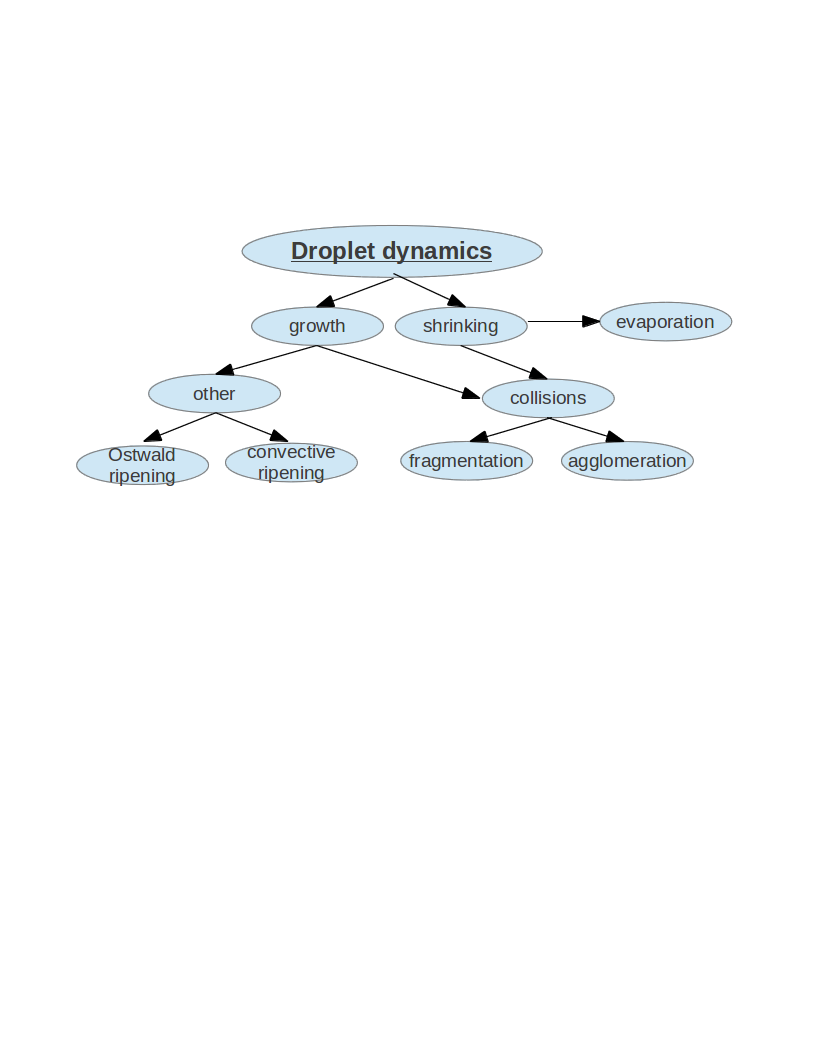
\includegraphics[width=\textwidth]{droplet_fig1.png}

\end{document}

